\documentclass[12pt, twoside]{book}

% Document Preamble: basic definitions and packages.
\usepackage[table]{xcolor}
\usepackage[english]{babel}
\usepackage[utf8]{inputenc}

% Page Margins and General Spacing
\usepackage[top=2.5cm, left=2cm, right=2cm, bottom=2.0cm]{geometry}
\usepackage{setspace}
\usepackage{xspace}


% Math-mode Coolness
\usepackage{amsmath}

% Variable Definition and Custom Commands
\newcommand{\titleEN}{Transparent Live Migration of Distributed Container Deployments in Userspace}
\newcommand{\projName}{\textsc{Cool System Name}\xspace}
\newcommand{\criu}{\textsc{CRIU}\xspace}
\newcommand{\redis}{\textsc{Redis}\xspace}
\newcommand{\runc}{\texttt{runC}\xspace}

% Comments by authors
\usepackage{ifthen}
\usepackage{amssymb}
\newboolean{showcomments}
\setboolean{showcomments}{true}
\ifthenelse{\boolean{showcomments}}
{ \newcommand{\mynote}[3]{
   \fbox{\bfseries\sffamily\scriptsize#1}
   {\small$\blacktriangleright$\textsf{\emph{\color{#3}{#2}}}$\blacktriangleleft$}}}
{ \newcommand{\mynote}[3]{}}
\newcommand{\jg}[1]{\mynote{Jordi}{#1}{blue}}
\newcommand{\cs}[1]{\mynote{Carlos}{#1}{red}}


% Graphics and TiKz
\usepackage{graphicx}
\usepackage{wrapfig} % Wrapping figures w/ text
\usepackage{tikz}
\usetikzlibrary{decorations.pathmorphing, patterns}
% We use this commands for sgx-principles.tex figure
\usepackage{pifont} % To use circled numbers in text
\newcommand*\blackcircled[1]{\tikz[baseline=(char.base)]{
            \node[shape=circle,fill,inner sep=0.5pt] (char) {\textcolor{white}{#1}};}}
\newcommand*\circled[1]{\tikz[baseline=(char.base)]{
            \node[shape=circle,draw,inner sep=2pt] (char) {#1};}}

% Headers, Footers and page numeration
\usepackage{fancyhdr}
% This is currently the default, change when placeholders TODO
%\fancyhead[LE,RO]{\slshape \rightmark}
%\fancyhead[LO,RE]{\slshape \leftmark}
%\fancyfoot[C]{\thepage}
%\pagestyle{fancy}
\fancypagestyle{frontmatter}{% Pagestyle for the frontmatter
  \renewcommand{\headrulewidth}{0pt}% No header rule
  \renewcommand{\footrulewidth}{0pt}% No footer rule
  \fancyhf[R]{\thepage}% Top right page number
  \fancyfoot{}%
}
\fancypagestyle{mainmatter}{%
  \renewcommand{\headrulewidth}{.4pt}% Header rule
  \renewcommand{\footrulewidth}{.0pt}% Footer rule
  %\fancyhf{}% Clear header/footer
  \fancyhead[LE]{\slshape\nouppercase{\leftmark}}% Chapter in header Left
  \fancyhead[RE]{\thepage}% Page number in header Right
  \fancyhead[LO]{\thepage}% Chapter in header Left
  \fancyhead[RO]{\slshape\nouppercase{\rightmark}}% 
  \fancyfoot{}
}
% The plain pagestyle is the one used by new Chapter pages and the ToC
\fancypagestyle{plain}{%
  \fancyhf{}%
  \fancyhead[R]{\thepage}
  \fancyfoot{}%
  \renewcommand{\headrulewidth}{0pt}% Line at the header invisible
  \renewcommand{\footrulewidth}{0pt}% Line at the footer visible
}

% Epigraph Package (Book Citation)
\usepackage{epigraph}
\setlength\epigraphwidth{.5\textwidth}

% Placeholders
\usepackage{lipsum}

% List of acronyms
\usepackage[toc,acronym,nomain,nonumberlist]{glossaries}

% Appendices
\usepackage[titletoc]{appendix}

% Code Listings Configuration
\usepackage{listings}
\definecolor{backcolour}{rgb}{0.95,0.95,0.92}
\lstset{ 
  backgroundcolor=\color{backcolour},   % Background color
  basicstyle=\scriptsize\ttfamily,        % the size of the fonts that are used for the code
  breakatwhitespace=false,         % sets if automatic breaks should only happen at whitespace
  breaklines=true,                 % sets automatic line breaking
  captionpos=b,                    % sets the caption-position to bottom
  commentstyle=\color{gray},    % comment style
  deletekeywords={...},            % if you want to delete keywords from the given language
  escapeinside={\%*}{*)},          % if you want to add LaTeX within your code
  extendedchars=true,              % lets you use non-ASCII characters; for 8-bits encodings only, does not work with UTF-8
  firstnumber=1,                % start line enumeration with line 1000
  frame=trbl,	                   % adds a frame around the code
  keepspaces=true,                 % keeps spaces in text, useful for keeping indentation of code (possibly needs columns=flexible)
  keywordstyle=\color{blue},       % keyword style
  morekeywords={*,println},            % if you want to add more keywords to the set
  numbers=left,                    % where to put the line-numbers; possible values are (none, left, right)
  numbersep=5pt,                   % how far the line-numbers are from the code
  numberstyle=\tiny\color{gray!80}, % the style that is used for the line-numbers
  rulecolor=\color{black},         % if not set, the frame-color may be changed on line-breaks within not-black text (e.g. comments (green here))
  showspaces=false,                % show spaces everywhere adding particular underscores; it overrides 'showstringspaces'
  showstringspaces=false,          % underline spaces within strings only
  showtabs=false,                  % show tabs within strings adding particular underscores
  stepnumber=1,                    % the step between two line-numbers. If it's 1, each line will be numbered
  stringstyle=\color{purple},     % string literal style
  tabsize=2,	                   % sets default tabsize to 2 spaces
  title=\lstname                   % show the filename of files included with \lstinputlisting; also try caption instead of title
}
% Syntax Highlighting for Scala
\lstdefinestyle{bash}{
    language = Bash,
    morekeywords={sudo,runc,criu,VBoxManage}
}
% Syntax Highlighting for Dockerfiles
\lstdefinelanguage{Dockerfile}{
  morekeywords={FROM, RUN, CMD, LABEL, MAINTAINER, EXPOSE, ENV, ADD, COPY,
    ENTRYPOINT, VOLUME, USER, WORKDIR, ARG, ONBUILD, STOPSIGNAL, HEALTHCHECK,
    SHELL},
  morecomment=[l]{\#},
  morestring=[b]"
}
% Syntax Highlighting for Docker Compose files
\lstdefinelanguage{docker-compose}{
  keywords={image, environment, ports, container_name, ports, volumes, links, user, command, build, depends_on},
  keywordstyle=\color{blue}\bfseries,
  identifierstyle=\color{black},
  sensitive=false,
  comment=[l]{\#},
  commentstyle=\color{purple}\ttfamily,
  stringstyle=\color{red}\ttfamily,
  morestring=[b]',
  morestring=[b]"
}
\renewcommand\lstlistlistingname{List of Listings}

% Hyphenation for \texttt
\usepackage[htt]{hyphenat}

% For nice looking tables
\usepackage{tabularx}
\usepackage{booktabs} % For the rules
\newcolumntype{L}[1]{>{\raggedright\arraybackslash}p{#1}}
\newcolumntype{C}[1]{>{\centering\arraybackslash}p{#1}}
\newcolumntype{R}[1]{>{\raggedleft\arraybackslash}p{#1}}

% References and \url
\usepackage{hyperref}

\usepackage{pdfpages}

% List of acronyms
\makeglossaries
\newacronym{api}{API}{Application Programing Interface}
\newacronym{blcr}{BLCR}{Berkeley Lab Checkpoint/Restart}
\newacronym{criu}{CRIU}{Checkpoint Restore in Userspace}
\newacronym{dmtcp}{DMTCP}{Distributed Multi-Threaded CheckPointing}
\newacronym{gid}{GID}{Group Identifier}
\newacronym{hpc}{HPC}{High Performance Computing}
\newacronym{isa}{ISA}{Instruction Set Architecture}
\newacronym{kvm}{KVM}{Kernel-based Virtual Machine}
\newacronym{lxc}{LXC}{Linux Containers}
\newacronym{oci}{OCI}{Open Container Initiative}
\newacronym{pid}{PID}{Process ID}
\newacronym{os}{OS}{Operating System}
\newacronym{pie}{PIE}{Position Independent Code}
\newacronym{pte}{PTE}{Page Table Entry}
\newacronym{qos}{QoS}{Quality of Service}
\newacronym{tcp}{TCP}{Transmission Control Protocol}
\newacronym{uid}{UID}{User Identifier}
\newacronym{vm}{VM}{Virtual Machine}
\newacronym{vmm}{VMM}{Virtual Machine Monitor}


\begin{document}
\onehalfspacing

\frontmatter
\pagestyle{frontmatter}

% MAMME mandatory cover

\includepdf[noautoscale=true, width=\paperwidth]{MAMME_Cover.pdf}
\newpage

% Title page
\thispagestyle{empty}
\begin{center}

    % FME - ETSETB
    
\includegraphics[height=2.1cm]{img/logo_fme.png} 
    \hfill
    
\includegraphics[height=2.1cm]{img/logo_ac.png}

    \vspace{0.5cm}

    % Joint work mention CFIS
    \Large
    \textsc{Technical University of Catalonia} 

    \textsc{School of Mathematics and Statistics - FME UPC}

    % Thesis Title
    \LARGE
    \rule{\textwidth}{0.4pt}
    \textbf{\titleEN}
    \rule[0.5cm]{\textwidth}{0.4pt}

    % Semester
    \vspace{-0.2cm}
    \Large
    \textsc{Spring Semester - July 2020}
    \vspace{0.7cm}

    % Author and Supervisors
    \normalsize
    \leavevmode\hbox to \linewidth{%
    \hspace{1cm}
    \begin{tabular}[t]{l@{}}
        \textit{Author:}  \\
        \textsc{Carlos Segarra Gonz\'alez\textsuperscript{1}} \\
        \texttt{carlos.segarra@estudiant.upc.edu}
    \end{tabular}
    \hfill
    \begin{tabular}[t]{l@{}}
        \textit{Supervisor:} \\
         \textsc{Jordi Guitart\textsuperscript{1,2}} \\
         \texttt{jguitart@ac.upc.edu} \\
    \end{tabular}%
    \hspace{1cm}
    }

    % Institutions
    \vspace{1cm}
    \footnotesize
    \textsuperscript{1} Universitat Polit\`ecnica de Catalunya BarcelonaTech, Barcelona, Spain

    \textsuperscript{2} Barcelona Supercomputing Center, Barcelona, Spain

    % Parial Fulfillment, ...
    \vspace{1.5cm}
    \normalsize
    In partial fulfillment of the requirements for the

    \textit{Master in Advanced Mathematics and Mathematical Engineering}

    % CSEM and CFIS
    \vfill
    
\includegraphics[height=2.1cm]{img/logo_upc.png}

\end{center}


% Blank page after title
\newpage
\thispagestyle{empty}
\null
\vfill
\pagebreak

% Epigraph TODO choose citation
\vspace*{2cm}
\epigraph{Like most of my generation, I was brought up on the saying: 'Satan finds some mischief for idle hands to do.' Being a highly virtuous child, I believed all that I was told, and acquired a conscience which has kept me working hard down to the present moment. But although my conscience has controlled my actions, my opinions have undergone a revolution. I think that there is far too much work done in the world, that immense harm is caused by the belief that work is virtuous, and that what needs to be preached in modern industrial countries is quite different from what always has been preached. Everyone knows the story of the traveler in Naples who saw twelve beggars lying in the sun (it was before the days of Mussolini), and offered a lira to the laziest of them. Eleven of them jumped up to claim it, so he gave it to the twelfth. This traveler was on the right lines. But in countries which do not enjoy Mediterranean sunshine idleness is more difficult, and a great public propaganda will be required to inaugurate it. I hope that, after reading the following pages, the leaders of the YMCA will start a campaign to induce good young men to do nothing. If so, I shall not have lived in vain.}{Bertrand Russell, \textit{In Praise of Idleness}}
\vfill
\pagebreak


% Blank page after epigraph
\newpage
\thispagestyle{empty}
\null
\vfill \pagebreak

% Note from the author TODO necessary? correctly placed?
\phantomsection
\addcontentsline{toc}{chapter}{Note from the Author}
\topskip0pt
\vspace*{4cm}
\Huge
\textbf{Note from the Author} \label{sec:acknowledgments}
\normalsize

\vspace{1cm}

The work here presented is my Master's Thesis for the Master in Advanced Mathematics and Statistics, from the School of Mathematics in the Technical University of Catalonia (FME-UPC).
It has been developed during a year-long collaboration with Jordi Guitart, from the Computer Architecture Department, who has lead the development and advised my research.
Part of this work has been funded by a research collaboration grant \textit{"Beca de Col$\cdot$laboraci\'o en Departaments Universitaris"} granted by the AGAUR from the regional government of Catalonia.

In particular, I have received a \textit{"BECA DE COL·LABORACI\'O EN DEPARTAMENTS UNIVERSITARIS - CURS 2019-2020"} funded by the \textit{"MINISTERIO DE EDUCACIÓN Y FORMACIÓN PROFESIONAL"}.

%\vspace{1cm}
%
%\begin{flushright}
%Carlos Segarra Gonz\'alez
%
%Neuch\^atel, \today
%\end{flushright}

\vspace*{\fill}


% Blank page after Note from Author
\newpage
\thispagestyle{empty}
\null
\vfill
\pagebreak

\phantomsection
\addcontentsline{toc}{chapter}{Declaration of Authorship}
\topskip0pt
\vspace*{4cm}
\Huge
\textbf{Declaration of Authorship} \label{sec:acknowledgments}
\normalsize

\vspace{1cm}

I hereby declare that, except where specific reference is made to the work of others, this Master's thesis has been composed by me and it is based on my own work.
None of the contents of this dissertation have been previously published nor submitted, in whole or in part, to any other examination in this or any other university.

\vspace{2cm}

Signed:

\rule[0.3cm]{.6\textwidth}{0.2pt}

\vspace{2cm}

Date:

\rule[0.3cm]{.6\textwidth}{0.2pt}


\vspace*{\fill}


% Blank page after Declaration of Autorship
\newpage
\thispagestyle{empty}
\null
\vfill
\pagebreak

% Acknowledgments
\phantomsection
\addcontentsline{toc}{chapter}{Acknowledgments}
\topskip0pt
\vspace*{2cm}
\Huge
\textbf{Acknowledgments} \label{sec:acknowledgments}
\normalsize

\vspace{1cm}

This work ends my Master in Advanced Mathematics and Mathematical Engineering and, at least for some years, my time at the Technical University of Catalonia.
I must admit that it does not feel as special as almost a year ago, when I was submitting my Bachelor's thesis.
It must be that I am getting used to it, or getting old, or maybe both.

In every personal success there's always a long list of people to be grateful, and I will try my best not to leave anyone out.

I will start the list with non-other than Jordi Guitart, my advisor.
I cold-emailed him a year ago and in the subsequent months he: has been flexible to adapt to my, sometimes picky, preferences.
Has helped me receive a grant to fund my work with him.
Has helped me in the arduous task of finding a PhD.
And overall has been a great advisor.
On the same line, I would like to thank the \textit{"Agencia de Gesti\'on de Ayudas Universitarias y de Investigaci\'on"} for the project funding.
Lastly, I must add some words for Juanjo Ru\'e, the Master's coordinator.
Right from the day I pre-enrolled he has always been welcoming, flexible, and responsive to all my concerns.

I would also like to take this moment to thank my parents for their relentless support, year in and year out.
This work ends a six-year-long chapter of my life, and kickstarts a new one at a different university, different city, and different country.
My last acknowledgment goes to those whose love I have learnt to appreciate thanks to a virus.
And sure they know who they are.

\vspace{1cm}

\begin{flushright}
Carlos Segarra Gonz\'alez

Barcelona, \today
\end{flushright}

\vspace*{\fill}


% Blank page after Acknowledgments
\newpage
\thispagestyle{empty}
\null
\vfill
\pagebreak

\phantomsection
%% ENGLISH VERSION ------------------------------------------------------------
\addcontentsline{toc}{chapter}{Abstract}
\topskip0pt
\vspace*{2.00cm}
\begin{center}
%    \large
%    UNIVERSITAT POLIT\`ECNICA DE CATALUNYA (UPC) 
%
%    \normalsize
%    Facultat de Matem\`atiques i Estad\'istica (FME)
%
%    Escola T\`ecnica Superior d'Enginyeria de Telecomunicaci\'o de Barcelona (ETSETB)
%
%    Centre de Formaci\'o Interdisciplin\`aria Superior (CFIS)
%
%    \vspace{0.5cm}
%
%    \large
%    SWISS CENTER FOR ELECTRONICS AND MICROTECHNOLOGY (CSEM)
%    \normalsize
%    Embedded Software Group - Systems Division
%    
%    \vspace{0.5cm}

    \LARGE
    \textit{\textbf{Abstract}} \label{sec:abstract}

    \vspace{0.5cm}

    \large
    \textbf{Using Trusted Execution Environments for Secure Stream Processing of Medical Data}

    by \textsc{Carlos Segarra Gonz\'alez}
\end{center}

\vspace{0.5cm}

\normalsize
Processing sensitive data, specially medical data produced by body sensors, on third-party untrusted clouds is particularly challenging without compromising the privacy of the users generating it. Typically, these sensors generate large quantities of continuous data in a streaming fashion. Such vast amount of information must be processed efficiently and securely, even under strong adversarial models. The recent introduction in the mass-market of consumer-grade processors with Trusted Execution Environments (TEEs), such as Intel SGX, paves the way to implement solutions that overcome less flexible approaches, such as those atop homomorphic encryption. 
    
This Bachelor Thesis presents a secure streaming processing system built on top of Intel SGX. To showcase the viability of this approach, we use it with a system specifically fitted for medical data. We design and fully implement a prototype system that we evaluate with several realistic datasets. Our experimental results show that our system introduces a reduced overhead to vanilla Spark while offering strong additional protection guarantees under powerful attackers and threat models.

\vspace{0.5cm}

\textbf{Keywords:} TEE, Trusted Hardware, Stream Processing, Intel SGX, Spark

\vfill
\pagebreak

%% CATALAN VERSION ------------------------------------------------------------
\topskip0pt
\vspace*{2cm}
\begin{center}
%    \large
%    UNIVERSITAT POLIT\`ECNICA DE CATALUNYA (UPC) 
%
%    \normalsize
%    Facultat de Matem\`atiques i Estad\'istica (FME)
%
%    Escola T\`ecnica Superior d'Enginyeria de Telecomunicaci\'o de Barcelona (ETSETB)
%
%    Centre de Formaci\'o Interdisciplin\`aria Superior (CFIS)
%
%    \vspace{0.5cm}
%
%    \large
%    SWISS CENTER FOR ELECTRONICS AND MICROTECHNOLOGY (CSEM)
%    \normalsize
%    Embedded Software Group - Systems Division
%    
%    \vspace{0.5cm}
%
    \LARGE
    \textit{\textbf{Resum}} 

    \vspace{0.5cm}

    \large
    \textbf{Using Trusted Execution Environments for Secure Stream Processing of Medical Data}

    per \textsc{Carlos Segarra Gonz\'alez}
\end{center}

\vspace{0.5cm}

\normalsize

El processat de dades de car\`acter personal, especialment aquelles provinents de dominis m\`edics, en servidors remots al n\'uvol, \'es particularment delicat quan es vol preservar la privacitat dels usuaris que les generen.
Molt habitualment, aquestes dades provenen de petits sensors que l'usuari du posats i que emeten un flux continu de mesures.
Dit volum de mesures no nom\'es han de ser processades de manera eficient, sin\'o tamb\'e de manera segura, fins i tot contra hipot\`etics atacants amb acc\'es privilegiat a les m\`aquines al n\'uvol.
La recent introducci\'o al mercat de processadors amb Entorns d'Execuci\'o Segura (\textit{Trusted Execution Environments}), com ara Intel SGX, faciliten la implementaci\'o de solucions m\'es flexibles i lleugeres que les basades en esquemes de criptografia homom\`orfica.
    
Aquest Treball de Final de Grau presenta una plataforma de processament segur de fluxos que es basa en Intel SGX.
Per il{\tiny\raisebox{.9ex}{\textbullet}}lustrar la viabilitat de la plataforma, la usem en un entorn m\`edic.
En el decurs del treball, dissenyem i implementem un sistema prototip que evaluem amb jocs de dades reals.
Els nostres resultats experimentals mostren que la plataforma introdueix un discret ralentiment en comparaci\'o amb la implementaci\'o est\`andard de Spark, tot oferint un nivell de protecci\'o adicional per a les dades dels usuaris. 

\vspace{0.5cm}

\textbf{Paraules Clau:} Entorns d'Execuci\'o Segura, Computaci\'o Segura, Processament de Fluxos, Intel SGX, Spark

\vfill


% Blank page after Abstract
\newpage
\thispagestyle{empty}
\null
\vfill
\pagebreak

% Table of contents: we prevent it from spanning more pages than required (default for two-paged documents is for the ToC to span a lot)
\pagestyle{plain}
\begingroup
\let\cleardoublepage\clearpage
\tableofcontents
\endgroup

\cleardoublepage
\phantomsection
\addcontentsline{toc}{chapter}{List of Figures}
\listoffigures

\cleardoublepage
\phantomsection
\addcontentsline{toc}{chapter}{List of Tables}
\listoftables

\cleardoublepage
\phantomsection
\addcontentsline{toc}{chapter}{\lstlistlistingname}
\lstlistoflistings

\glsaddall
%\addcontentsline{toc}{chapter}{List of Acronyms}
\printglossary[type=\acronymtype,title=List of Acronyms]

\mainmatter
\pagestyle{mainmatter}
% Main Chapters
\chapter{Introduction} \label{chap:introduction}


\chapter{Background Concepts} \label{chap:background}

\section{Containers} \label{sec:containers}

Jordi, you might add comments using \texttt{\textbackslash jg} command \jg{like this}.

An Introduction to containers, what are they used for, some data, ...

\subsection{An Introduction to Virtualization}

Virtualization is a recurrent technique in systems design in computer science which aims to provide processes the illusion that they interact with a defined interface, hiding the real implementation behind.
Some of the most relevant features facilitated by virtualization are: process isolation from other processes and the underlying system, fine-grained dynamic resource provisioning, multiple virtually dedicated subsystems on the same physical instance, among others.
We classify virtualization techniques according to the type of interface being virtualized.

\textbf{Emulation.}
Emulators allow applications written for a certain computer architecture to run on a different one.
They do so by translating (\textit{i.e.} virtualizing) the Instruction Set Architecture (ISA).
An example of such a system is \textsc{Qemu} (\url{https://www.qemu.org/}).

\textbf{Hardware Virtualization.}
Hardware virtualization interfaces a complete system which enables to run a fully-featured operating system within a different one.
It has traditionally been one of the most user-friendly virtualization tools in the form of \emph{virtual machines} such as the Linux-Kernel Virtual Machine \textsc{KVM} (\url{https://www.linux-kvm.org/page/Main_Page}, \textsc{VMWare Workstation} (\url{https://www.vmware.com/}) or Oracle's \textsc{VirtualBox} (\url{https://www.virtualbox.org/}).
We differentiate between full virtualization and paravirtualization.
The former adds an hypervisor or virtual machine monitor (VMM) which creates the illusion of multiple virtual machines, which are multiplexed across the physical resources, and allow to run an \emph{unmodified} guest OS.
The latter modifies the guest OS' source code and replaces sensitive calls with \emph{hypercalls}, which are direct calls to the hypervisor.

\textbf{OS-level Virtualization.}
Operating Sytem-level virtualization allows for multiple isolated user-space instances, called \textbf{containers} which share a single operating system.
In comparison to traditional virtual machines, containers add little overhead, require minimal startup, and have a low resource requirement, all this factors make them highly scalable.
Containers have experienced an exponential increase in usage, specially with the advent of open-source highly-available container engines such as \textsc{Docker} (\url{https://www.docker.com/}), Linux Containers \textsc{LXC} (\url{https://linuxcontainers.org/}), \textsc{Podman} (\url{https://podman.io/}, among others.
Given that the goal of this project is to perform efficient live migration of running containers, the following section provides further technical details on containerization.

\subsection{Working Principles of Containers}

As previously introduced, a linux container is a set of processes that are isolated from the rest of the machine.
To achieve this isolation, they rely on two kernel features: control groups and namespaces~\cite{namespaces-manual}.

\subsubsection*{Namespaces}

As greatly phrased by Michael Kerrisk in his series of articles on namespaces~\cite{Kerrisk2013}, the purpose of namespaces is to wrap a global system resource and abstract it in a way that each process within the namespace thinks it has its own isolated instance of such resource.
As of Kernel 5.6, there are eight different types of namespaces, which we present together with a brief description and their respective flag in Table~\ref{table:namespaces}.
\begin{table}[h!]
    \centering
    \rowcolors{1}{gray!20}{}
    \begin{tabular}{p{2cm}p{13cm}}
        \hline
        \textbf{Kind} & \textbf{Description} \\[3pt]
        \hline \hline
        \texttt{mnt} & \textbf{Mount namespaces} provide isolation of the list of mount points seen by the process in each namespace instance. It allow processes to have their own root file system and mount and unmount file systems without affecting the rest of the system. \\[3pt]
        \texttt{pid} & The \textbf{process ID} isolates the PID number space. This means that two processes in different PID namespaces can have the same identifier. It is very useful in container migration as it allows to restore the processes with the same PID they were dumped with regardless of whether that ID might be taken in the target machine or not. \\[3pt]
        \texttt{net} & \textbf{Network namespaces} provide isolation of the whole network stack. In particular network devices, interfaces, routing tables, iptables rules, and sockets. \\[3pt]
        \texttt{ipc} & The \textbf{Interprocess Comunication namespace} provides isolation for POSIX semaphore queues, semaphore sets and shared memory segments.\\[3pt]
        \texttt{uts} & The \textbf{UNIX Time Sharing namespace} allows processes to set a hostname or domainname for that particular namespace without affecting the rest of the system. \\[3pt]
        \texttt{user} & \textbf{User namespaces} isolate security-related identifiers such as user and group identifiers (UID, GID) and capabilities. This allows for a process to have privileges within a certain namespace but not outside it's scope. \\[3pt]
        \texttt{cgroup} & The \textbf{Control Group namespace} virtualizes the contents of \texttt{/proc/self/cgroup}. As a consequence each different namespace has a different cgroup root directory.\\[3pt]
        \texttt{time} & The \textbf{time namespace} has been the latest addition to the group. Included in Kernel 5.6, it allows different namespaces to have different offsets to the system monotonic and boot-time clock.\\[3pt]
        \hline
    \end{tabular}
    \caption[List of the different namespaces supported in Kernel 5.6.]{List of the different namespaces supported in Kernel 5.6. and a brief description of the isolation they provide.\label{table:namespaces}}
\end{table}
In order to create a new namespace of a given time, we can follow two approaches.
With the \texttt{clone} system call, we can create a new child process, in a similar way to \texttt{fork} but with higher control of what pieces of execution context are inherited~\cite{clone-manual}.
More specifically, with the \texttt{unshare} system call we can specifically unshare a namespace from parent process~\cite{unshare-manual}.
To join an existing namespace, we can use the \texttt{setns} syscall, which given a file descriptor referring to a namespace, it links the calling process to it.~\cite{setns-manual}.
These operations require the \texttt{CAP\_SYS\_ADMIN} capability.
In Listings~\ref{code:namespaces-unshare} and~\ref{code:namespaces-setns} we include examples of usage of \texttt{unshare} and \texttt{setns} respectively.
\begin{figure}[h!]
    \begin{minipage}{.45\textwidth}
        \begin{lstlisting}[language=C,caption={Snippet to unshare the calling thread from a namespace using the \texttt{unshare} system call.\label{code:namespaces-unshare}}]
#define _GNU_SOURCE
#include <errno.h>
#include <sched.h>
#include <stdio.h>

// Unshare from parent namespace
int main(int argc, char *argv[])
{
    /* Available flags:
     * CLONE_NEWCGROUP, CLONE_NEWIPC
     * CLONE_NEWNS, CLONE_NEWNET
     * CLONE_NEWPID, CLONE_NEWTIME
     * CLONE_NEWUTS, CLONE_NEWUSER
     */
    flags = CLONE_NEWNET || CLONE_NEWPID;

    if (unshare(flags) == -1)
    {
        perror("unshare failed");
        exit(EXIT_FAILURE);        
    }

    return 0;
}
\end{lstlisting}
    \end{minipage} \hfill
    \begin{minipage}{.45\textwidth}
        \begin{lstlisting}[language=C,caption={Scripts to perfrom two pre-dumps and a dump of a running process using CRIU.\label{code:namespaces-setns}}]
#define _GNU_SOURCE
#include <errno.h>
#include <sched.h>
#include <stdio.h>

// Attach calling process to an existing
// network namespace.
int main(int argc, char *argv[])
{
    // Get namespace FD
    fd = open("/proc/330/ns/net", O_RDONLY);

    // Join the namespace
    if (setns(fd, CLONE_NEWNET) == -1)
    {
        perror("setns failed");
        exit(EXIT_FAILURE);        
    }

    return 0;
}
\end{lstlisting}
    \end{minipage}
\end{figure}

\subsubsection*{Control Groups}

Control groups (\texttt{cgroups}) are a resource management kernel feature that allows handling of processes in hierarchical groups.
This way, fine-grained resource metering and limiting can be applied on a per-group basis.
Typical resources monitored using this technique are memory, CPU usage, I/O network, among others.

These constraints are enforced through the usage of kernel subsystems.
Each different subsystem, mapped to one of the resources to manage, has an independent hierarchy.
Each process then belongs to exactly one group per subsystem.
For instance, the memory cgroup keeps track of the pages used and imposes different limits for physical, kernel, and total memory.

\subsection*{Container Terminology}

With the rapid increase in popularity, a wide-range of terminology has also been introduced in the container ecosystem.
These terms are commonly misused~\cite{McCarty2018} and, even though they don't cover the technical principles, are useful to differentiate the services different tools offer.

A \emph{container} is the (set of) isolated Linux process.
It is a running instance of a \emph{container image}, a (set of) files that are used locally as a mount point.
To enhance portability and vendor interoperability, images are stored using a standardized format by the Open Container Initiative (OCI, \url{https://opencontainers.org/}), an open governance structure for container-related standards.
The \emph{container engine} turns the image into a running container and acts as the interaction point with the user.
However, engines don't tend to actually instantiate the containers themselves, and rather rely on a \textit{container runtime}.
The runtime is the lower level component that interacts with the kernel, it's specification~\cite{container-runtime-specification} is also maintained and developed by the OCI.
\runc is it's reference implementation, and our tool of choice to implement live migration.
We have chosen to skip the engine layer and interact with the runtime as support for advanced \criu features is lacking in higher-level tools.

\subsubsection*{Different Container Engines and Runtimes}

Differnt container engines

Different container runtimes: crun, railcar and katacontainers (no runc)
Docker, CRI-O, and others runc.

\subsubsection*{\runc: the reference runtime implementation}

Originally developed at Docker, \runc is a lightweight container runtime aimed to provide low-level interaction with containers.
In 2015~\cite{introducing-runc}, Docker open-sourced the component and transferred ownership to the Open Container Initiative (OCI), who has since then lead the project in a fashion similar to that of the Linux Foundation.
Since then, several container engines such as \textsc{Podman} (\url{https://podman.io/}) and \textsc{CRI-O} (\url{https://cri-o.io/}) have made \runc their runtime of choice.

The OCI has since then released specifications for container runtimes, engines, images, and image distribution.
\runc is nowadays an OCI-compliant container runtime (it is, in fact, the reference implementation).

Users are encouraged to interact with containers through container engines, but \runc itself provides an interface to create, run, and manage containers natively.
Integration with \criu has to be done on a per-project basis, and \runc has the most advanced and stable integration.
Therefore, we decided to use it to manage our containers.

Running a container with \runc is slightly different than doing it in, let's say, Docker, as the user's interaction with the underlying system is more direct.
In particular, in \runc there is no notion of \textit{images}.
To run a container, a user must provide a specification file (\texttt{config.json}) and a root file system in a directory (\texttt{rootfs}).
Through the specification file several low-level options such as namespaces, control groups, and capabilities can be configured.

\section{Checkpointing}

Brief introduction, what is checkpointing

\subsection{Checkpoint-Restore}

\subsection{Live Migration}

Iterative, pre-copy, post-copy, ... \cite{Clark2005}

\subsection{Distributed Checkpointing}

\section{\criu: Checkpoint Restore in Userspace}

Checkpoint/Restore in Userspace (\criu) is an open-source C/R tool~\cite{criu-main-page}.
Introduced in 2011, it's distinctive feature is that it is mainly implemented in user space, rather than in the kernel, by using existing interfaces~\cite{Reber2016}.
One of the most important interface is \texttt{ptrace}~\cite{ptrace-manpage}, as it relies on it for seizing the target process.
For other interfaces, several patches have been pushed to the mainline kernel by \criu developers~\cite{criu-kernel-patches}.
The project is currently under active development~\cite{criu-github}, and its main focus is to support the migration of containers.

\subsection{A Technical Overview on \criu}

The main goal of \criu is to perform a snapshot the current process' tree state to a set of image files, so that it can be later restored that exact point in time, without reproducing the steps that led to it.

\subsubsection*{Checkpoint}

The checkpointing process starts with the process identifier (PID) of a process group leader provided by the user through the command line using the \texttt{--tree} option~\cite{criu-checkpoint}.
However, before it can actually start, we need to ensure that the process does not change it's state during checkpoint.
This includes: opening file descriptors, changing sessions, or even producing new child processes~\cite{criu-freeze}.
To achieve this transparently, instead of sending a stop signal (which could affect the process' state) \criu freezes tasks using \texttt{ptrace}'s \texttt{PTRACE\_SEIZE} command~\cite{ptrace-manpage}.
In order to find all active tasks descendant of the parent PID, the \texttt{\$pid} dumper iterates through each \texttt{/proc/\$pid/task/} entry, recursively gathering threads and their children from \texttt{/proc/\$pid/task/\$tid/children}.

Once all tasks are frozen, \criu collects all the information it can about the task's resources.
File descriptors and registers are dumped through a \texttt{ptrace} interface and are parsed from \texttt{/proc/\$pid/fd} and \texttt{/proc/\$pid/stat} respectively.
In order to dump the contents of memory and credentials, a novel technique is introduced, the \textbf{parasite code}.

The parasite code is a binary blob built as a position independent executable (PIE) for execution inside another process adress space.
It's purpose is to execute \criu calls from within the dumpee's task address space~\cite{criu-parasite-code}.
To achieve this goal, \criu must:
\begin{enumerate}
    \item Move task into seized state calling \texttt{ptrace(PTRACE\_SEIZE, ...)}. Note that the task is stopped without it noticing, hence not altering it's state.
    \item Inject an \texttt{mmap} syscall in the current stack's instruction pointer, and allocate memory for the whole code blob. At this stage, space for exchanging parameters and results is also allocated within the dumpee's process adress space. \criu is now ready to run parasite service routines.
    \item The external dumping process retrieves information about the dumpee's adrress space through the parasite code either through \emph{trap} mode (one command at a time) or \texttt{daemon} mode (in which the parasite behavies as a UNIX socket.
    \item With information about used memory areas and important flags read from \texttt{/proc/\$pid/smaps/} and \texttt{/proc/\$pid/pagemap}, the parasite code transfers the actual content outside through a set of pipes, which in turn gets translated into image files.
\end{enumerate}
Lastly, the target process is cured from the parasite by closing it, unmapping it's allocated memory area, and reverting to the original frozen state.

\subsubsection*{Restore}

During the restore process, \criu morphs into the to-be-restored task.
Since we checkpoint process trees rather than single processes, \criu must \texttt{fork} itself several times to recreate the original PID tree.
In particular, and in order to be completely transparent, \criu requires that the restored tasks have the same PID they had before dump.
To achieve this goal, older versions of \criu had to perform very time-sensitive and race condition-prone PID handling, what was referred to as the PID dance~\cite{Reber2019,criu-pid-dance}.
Starting with kernel 5.3 and the new \texttt{clone3()} system call, it becomes now possible to clone a process and specify the desired PID for it~\cite{kernel-clone3}.

Then \criu restores all basic task resources such as file descriptors, namespaces, maps, ...
The only resources that are \emph{not} restored at this stage are, most notably, memory mappings.
In order to restore memory areas, and since the morphing is done \textit{in-place}, before exitting \criu would have to unmap itself and map the application code.
To overcome this issue, a similar approach to the parasite code one is followed, the \textbf{restorer blob}.
The restorer blob is a piece of PIE code, to which \criu transfers control to unmap itself and map the appropriate code and memory areas for the process to restore successfully.

\subsubsection*{Live Migration with Criu}

TO-DO

\subsection{Comparison with Other C/R Tools}

We can beneffit from this table:

- \url{https://criu.org/Comparison_to_other_CR_projects}

Compare:

- VM C/R

- CRIU

- DMTCP

- BLCR

- FTI: maybe this falls a bit out of the scope \url{https://github.com/leobago/fti}

We could also include snippets of how to run a Hello World for each alternative.


\chapter{Related Work} \label{chap:related-work}

I would like to organize this chapter in several sections, for the moment I will dump the references I have been gathering:

\textbf{Distributed Algorithms:}

Distributed Algorithms for Message-Passing Systems~\cite{Raynal2013}

Distributed Computing: Principles, Algorithms, and Systems~\cite{Kshemkalyani2008}

\textbf{Checkpoint Restore:}

Autosave for Research: Where to Start with Checkpoint/Restart~\cite{Barker2014}

Checkpoint-restart for a network of virtual machines~\cite{Garg2013}

\textbf{CRIU:}

CRIU and the PID dance~\cite{Reber2019}

Fast In-Memory CRIU for Docker Containers~\cite{Venkatesh2019}

\textbf{Live Migration:}

Live Migration of Virual Machines~\cite{Clark2005}

\textbf{DMTCP:}

DMTCP: Transparent Checkpointing for Cluster Computations and the Desktop~\cite{Ansel2009}.

MANA for MPI: MPI-Agnostic Network-Agnostic Transparent Checkpointing~\cite{Garg2019}

\textbf{Other:}

Distributed Checkpointing with Docker Containers in High Performance Computing (thesis)~\cite{Berg2017}

MPICH-V: Toward a Scalable Fault Tolerant MPI for Volatile Nodes~\cite{Bosilca2002}.

Live Service Migration in Mobile Edge Clouds~\cite{Machen2018}

\chapter{\projName (think of a name for the system)} \label{chap:system}

In this chapter we present our implementation of live migration of \runc containers using \criu.
In order to achieve efficiency, liveness, and mimick a realistic setting, we explore disk-less and iterative migrations, and checkpointing established TCP connections and external namespaces.
First, in \S\ref{sec:arch-blocks}, we cover the implementation of each of these features in \criu and their integration with \runc.
Then, we perform a set of microbenchmarks to assess their impact on performance, and finish with a snippet showcasing their usage.
Lastly, in \S\ref{sec:system}, we provide insights on our final open source implementation available at \url{https://github.com/live-containers/live-migration}.

\section{Building Blocks} \label{sec:arch-blocks}

In this first section we study the implementation of diskless and iterative migration in \criu.
The former allows fast checkpoint/restore without writing to disk.
The latter allows for incremental dumps, which in turn reduces downtime when migrating an application as the load can be divided among subsequent dumps.
We also introduce how to checkpoint and migrate established TCP connections and established namespaces.

For each different feature, we prepare a set of experiments.
Unless otherwise stated, we run each one in a Debian machine with kernel version \texttt{4.19.0-6} and use \criu version 3.13 and \runc version \texttt{1.0.0-rc8}, both built from source.

\subsection{Diskless Migration}

As previously detailed, \criu builds the snapshot of a running process using image (\texttt{.img}) files, which are stored in a user-specified path.
As a consequence, it relies heavily on the underlying storage facility provided which, in most commodity PCs, tends to be the disk-backed file system.
It is of no surprise then, that reading and writing from and to disk can quickly become the bottleneck in live migration performance.
It gets even worse when writes are duplicated, \textit{i.e.} we write once to disk to dump the process state, and a second time to transfer image files wherever they need to be restored.
To overcome the former, we rely on \texttt{tmpfs} a virtual memory filesystem~\cite{tmpfs-manpage}.
For the latter, we leverage \criu's \texttt{page-server}.

% TMPFS
First presented by Sun Microsystems in 2007~\cite{Snyder2007}, \texttt{tmpfs} is a memory-based file system that uses resources from the virtual memory subsystem.
According to the Linux Programmer's Manual~\cite{tmpfs-manpage}, this file system can employ swap space if memory pressure is high, only consumes as much memory as required to store the current files (regardless of the allocated size), and unmounting it destroys the contents therein.
Since the files actually reside in memory, the user benefits from memory-like read/write performance.
A notable use of \texttt{tmpfs} is \texttt{/dev/shm}, used in the POSIX-compliant implementation of shared memory and in POSIX semaphores.
One such file system can be easily created and destroyed using \texttt{mount} and \texttt{umount} as detailed in Listing~\ref{code:tmpfs-example}
\begin{lstlisting}[style=Bash,caption={Mounting and dismounting a \texttt{tmpfs} filesystem.\label{code:tmpfs-example}}]
#!/bin/bash
# Mount a tmpfs filesystem rooted in the /tmp/my-tmpfs directory with maximum size 100 MB
mkdir /tmp/my-tmpfs
sudo mount -t tmpfs -o size=100M tmpfs /tmp/my-tmpfs

# Check the new file system appears in the list of mounted devices
sudo mount | grep /tmp/my-tmpfs

# Unmount the filesystem 
sudo umount /tmp/my-tmpfs # CAUTION: THIS WILL DESTROY THE CONTENTS
\end{lstlisting}

% Page-server
The page server is a component of \criu that allows to send memory dumps directly through the network, saving disk read/writes on the origin, writing them once they reach the destination system~\cite{criu-page-server}.
Note that the page server is used only to migrate memory files, which tend to be the largest ones, whereas other image files still need to be transferred when migrating.
The current implementation uses only TCP sockets and no encryption nor compression is used on the network transfer.
It is also worth mentioning that \texttt{criu page-server --port} is a one-shot command, \textit{i.e.} if we perform multiple dumps, a page server must be started for each one of them.
Observe that, even though it introduces a small overhead, our results (see Figure~\ref{fig:diskless-migration-microbenchmark}) show that for migrations within the same machine, setting up a page server in $\texttt{localhost}$ outperforms the double-copying approach for larger applications.

% Integration w/ runC
As introduced in the previous paragraphs, the key pieces to achieve efficient diskless migrations are making use of a \texttt{tmpfs} file system and \criu's page server.
The former is in another level of abstraction than \runc, and for the latter we need to start the page server separately and then checkpoint passing address and port as a parameter to the \texttt{--page-server} flag.
In Listings~\ref{code:microbenchmark-diskless-runc} and~\ref{code:microbenchmark-diskless-criu} we include snippets to perform a checkpoint with a page server using \runc and \criu respectively.
\begin{figure}[h!]
\begin{minipage}{.45\textwidth}
\begin{lstlisting}[style=Bash,caption={Commands to perform a checkpoint in \runc using a page server.\label{code:microbenchmark-diskless-runc}}]
#!/bin/bash
# Start the Page Server
sudo criu page-server \
    --port 9999 \
    --images-dir /path/to/dst/images &

# Checkpoint using the page-server
sudo runc checkpoint \
    --image-path /path/to/src/images \
    --page-server 127.0.0.1:9999 \
    <container_name>

# To finish the migration we would need to
# copy the remaining files
# This should be fast as memory dumps are 
# already at destination
cp /path/to/src/images/* \
    /path/to/dst/images/
\end{lstlisting}
\end{minipage}\hfill
\begin{minipage}{.45\textwidth}
\begin{lstlisting}[style=Bash,caption={Commands to perform a checkpoint in \criu using a page server.\label{code:microbenchmark-diskless-criu}}]
#!/bin/bash
# Start the Page Server
sudo criu page-server \
    --port 9999 \
    --images-dir /path/to/dst/images &

# Checkpoint using the page-server
sudo runc checkpoint \
    --image-path /path/to/src/images \
    --page-server 127.0.0.1:9999 \
    <container_name>

# To finish the migration we would need to
# copy the remaining files
# This should be fast as memory dumps are
# already at destination
cp /path/to/src/images/* \
    /path/to/dst/images/
\end{lstlisting}
\end{minipage}
\end{figure}

% Experiment
In order to benchmark the performance of diskless migration when compared to disk-based one and the benefits of using a page server, we set up two different experiments.
In one hand we have a counter program written in C (see Listing~\ref{code:c-counter} for the full implementation) that increments a value and prints it to \texttt{stdout}.
On the other hand we have an instance of a \redis in-memory database that we pre-load with $1e7$ keys.
The total weight of the memory image dump is $912$ MB.
For each experiment, we measure the time to checkpoint the process and transfer the remaining images to a different directory, either locally or on a different machine in the same local network.
We compare the performance when using \texttt{tmpfs} directories to store the images (diskless) or not (file-based) and when using a page server or not.
Each test is run 100 times and we present the average and standard deviation values obtained in Figure~\ref{fig:diskless-migration-microbenchmark}.

% Results
\begin{figure}[h!]
    \centering
    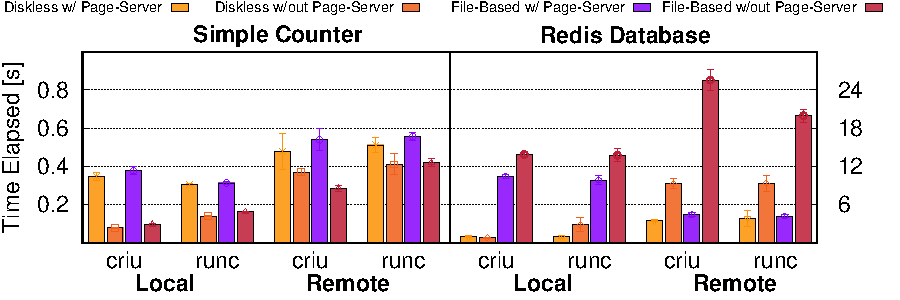
\includegraphics[width=.8\textwidth]{figs/diskless-migration-microbenchmark/diskless_migration_microbenchmark.pdf}
    \caption[Size of the memory image for iterative dumps.]{Time elapsed checkpointing and migrating a running process when using file-based or diskless migration, with and without a page server. We compare the results for a small application (around 100 kB, left) and a big one (around 1 GB, right).\label{fig:diskless-migration-microbenchmark}}.
\end{figure}

The first and most important conclusion we draw from our results is that there is no one-size-fits-all solution when choosing the best setting to migrate our application.
It seems clear that diskless is always equal or better than non-diskless.
This was to be expected, as for the same setting, \texttt{tmpfs} gives better raw read/write performance.
For instance, when transferring image files from one machine to the other, the perceived end-to-end throughput between \texttt{tmpfs} directories is in the order of 100-120 Mbps compared to the 60-70 Mbps for regular directories.
However, there might be situations, or systems, which simply don't have that much free memory.
The Redis dump files alone already take up 1 GB of memory, unacceptable in constrained devices.

If the application is sufficiently small (a dump for an instance of the counter process is around 90 kB), the overhead of running a page server is higher than simply writing the files twice, both in the local and remote setting.
However, for large applications, diskless outweighs the page server in the local case, whereas if we have to send files over the network, running a page server is more important than using the diskless approach (although a combination of both yields the best performance).
We include the full evaluation scripts in Listing~\ref{code:microbenchmark-diskless-evaluation}.

\subsection{Iterative Migration}

% Brief Introduction
%As introduced in \S

Implemented in \criu we find a series of features that enable us to perform iterative migrations of running processes.
This is, periodically snapshot the state of the process without altering it until some condition is triggered, that in turn checkpoints the container and restores it elsewhere.
The key idea being that all the heavy work for the snapshot (\textit{i.e.} capturing the memory state and transferring it) will have already been done in previous iterations, hence minimizing the application downtime.

In the previous paragraph we have assumed that transfers across consequent snapshots will be smaller in size, otherwise the $n$-th dump would not be any faster than the first one, and we would be wasting a lot of bandwidth since the same information would be sent repeatedly.
This reduction in size can be achieved through memory tracking, a procedure through which memory pages written between dumps are marked as \emph{dirty} and hence included in the following transfer.
Therefore, to implement efficient iterative migration we need:
\begin{enumerate}
    \item \textbf{Pre-Dump:} A procedure to snapshot the memory of the process without stopping it (note that, at this point, we don't need all the other details).
    \item \textbf{Memory Tracking:} A procedure to keep track of the memory changes in a process' address space.
    \item \textbf{Parent Directory:} A procedure to link together subsequent dumps so that they can be correctly re-interpreted at restore time.
\end{enumerate}

The first step during an iterative migration consists on dumping \emph{all} of the process memory to an image file.
This allows for a baseline from which smaller \emph{incremental} dumps are performed.
Note that, at this point, we are not interested in capturing the whole state, hence the usage of the \texttt{pre-dump} command in CRIU.

Memory tracking in CRIU~\cite{criu-memory-tracking} is done by means of a kernel functionality introduced in 2013~\cite{criu-memory-tracking-lwn}.
It consists of two steps: first we ask the kernel to keep track of memory changes on a per-process basis by writing a $4$ to \texttt{/proc/\$pid/clear\_refs} and, after a while, reading the \texttt{/proc/\$pid/pagemap} file and checking the \textit{soft-dirty} bit for each page table entry (PTE).
Internally, in the first step the kernel clears all soft-dirty bits \emph{and} the writable ones per each PTE for the given process id (PID).
Subsequent writes to any page will trigger a page fault, a call to \texttt{pte\_mkdirty}, and therefore the \textit{soft-dirty} bit will be set.
During the second step, at memory dump time, if this bit has not been set, the memory page needs not to be transferred again.
To enable this functionality in \criu, we must use the \texttt{--track-mem} flag.

One last key step required to achieve efficiency and correctness upon restore is to link the actual dump (or pre-dump) with the one preceding it, it's \emph{parent}.
For a pre-dump, \texttt{--prev-images-dir} indicates \criu to look for existing dumps in the specified path, and perform the bit-checking described in the previous paragraphs.
Upon restore, links among successive dumps are pieced together to successfully restore the freshest version of the running program.

The integration with \runc is seamless.
The pre-dump functionality is triggered with the \texttt{--pre-dump} flag which, in turn, sets the memory tracking flag automatically~\cite{runc-memtrack}.
Lastly, the \texttt{--parent-path} flag can be used to achieve the correct linkage between dumps.
In Listings \ref{code:microbenchmark-iterative-criu} and \ref{code:microbenchmark-iterative-runc} we include the different scripts to perform the three consecutive dumps both in \criu and \runc.
The complete scripts used for the benchmarking are included in Listing \ref{code:microbenchmark-iterative-evaluation}.
\begin{figure}[h!]
\begin{minipage}{.45\textwidth}
\begin{lstlisting}[style=Bash,caption={Scripts to perform two pre-dumps and a dump of a running process using CRIU.\label{code:microbenchmark-iterative-runc}}]
#!/bin/bash
# First Pre-Dump
sudo runc checkpoint \
    --pre-dump \
    --image-path ./images/1/ \
    <container_name>

sudo runc list # Container running

# Second Pre-Dump
sudo runc checkpoint \
    --pre-dump \
    --parent-path ../1/ \
    --image-path ./images/2/ \
    <container_name>

sudo runc list # Still running

# Last Dump
sudo runc checkpoint \
    --parent-path ../2/ \
    --image-path ./images/3/ \
    <container_name>

# Container is now stopped
\end{lstlisting}
\end{minipage}\hfill
\begin{minipage}{.45\textwidth}
\begin{lstlisting}[style=Bash,caption={Scripts to perform two pre-dumps and a dump of a running container using runC.\label{code:microbenchmark-iterative-criu}}]
#!/bin/bash
# First Pre-Dump
sudo criu pre-dump \
    -t  PROCESS_PID \
    --images-dir images/1 \
    --track-mem \
    --shell-job 

# Second Pre-Dump
sudo criu pre-dump \
    -t PROCESS_PID \
    --shell-job \
    --images-dir images/2 \
    --prev-images-dir ../1 \
    --track-mem

# Last Dump
sudo criu dump \
    -t  PROCESS_PID \
    --images-dir images/3 \
    --prev-images-dir ../2 \
    --shell-job \
    --track-mem

# Process is now stopped
\end{lstlisting}
\end{minipage}
\end{figure}

\jg{Mention somewhere that a threshold defines for how long the migration iterates on copying dirty memory before deciding to stop the container and do the final copy. This is probably a parameter that one can play with to tune the migration process (although we don't evaluate this in our experiments).}

In order to perform a micro-benchmark of this functionality we consider two different scenarios: a simple counter written in \texttt{C}, and a \redis in-memory database, as introduced in the previous section.
For each scenario we perform two pre-dumps, and a final dump, and report the size of the \texttt{pages-1.img} file (which contains the memory dump).
We test a static setting in which we don't change the memory during successive dumps which acts as a baseline, and a dynamic one in which, between each dump, we modify the contents of the process memory.
For the counter, the static setting starts the program and goes to sleep, whereas the dynamic one indeed updates the counter every other second.
For the database, we initially pre-load it with $1e7$ key-value pairs (around 300 MB of data) and then either do nothing, or run a \texttt{redis-benchmark} which alters around $1\%$ of the key pairs.
Lastly, we compare the results of running the experiments with vanilla \criu or through \runc.

\begin{figure}[h!]
    \centering
    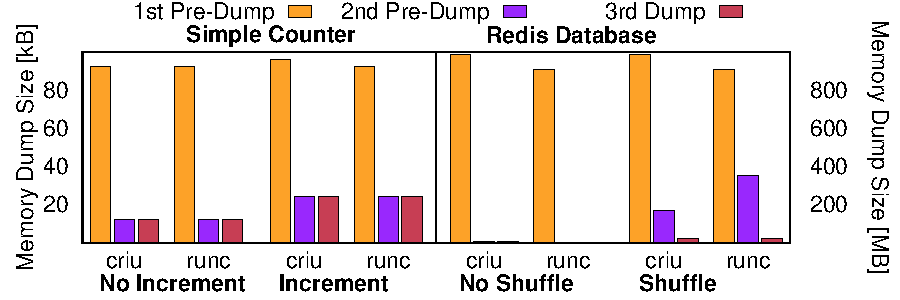
\includegraphics[width=.8\textwidth]{figs/iterative-migration-microbenchmark/iterative_migration_microbenchmark.pdf}
    \caption[Size of the memory image for iterative dumps.]{Size of the dumped memory image when performing iterative dumps. For the counter experiment we report the results in kB (left axis) and for the redis one we report the results in MB (right axis). We compare the results when using \runc or purely \criu.\label{fig:iterative-migration-microbenchmark}}.
\end{figure}

We present our results in Figure~\ref{fig:iterative-migration-microbenchmark}.
First of all, note how we use different scales for the counter application (left) and the \redis one (right).
We observe that, as expected, if we make no changes to the process' memory after the first dump, the amount of information to be re-transferred is very little, which we attribute it to \criu's metadata.
In the counter case, the initial dump is around 90 kB and subsequent ones are 12 kB, whereas in the \redis one, the size decreases from 900 MB to just 1 MB.
Once we modify the memory, additional pages need to be transferred.
In the counter case, between successive dumps we just increase the value of a variable and alter the state of \texttt{stdout}, what translates in a 10 kB increase in the image size every time.
In the \redis one, the \texttt{redis-benchmark} is non-deterministic in nature, but it's worth observing how shuffling a percent of the total key-store propagates to higher percentages of memory re-use.
We conclude that memory tracking is a necessary feature if any application considers even near-live migration of production applications, and the technology presented allows for an easy way to do-so.


\subsubsection*{Aside: Memory Deduplication}

Maybe not an aside, but putting it here to remember

\cs{Mention that before we were optimizing a-priori, whereas this technique is a-posteriori.}

%\subsection{Remote Migration}
% CS: I forgot to comment this. I initially included it but then figured out it did not add any value since the main difference would be raw bandwidth.
%\jg{I assume you will place here some experiments demonstrating the migration between different nodes?}

\subsection{Checkpointing TCP Connections}

The ability to checkpoint established TCP connection is mainly due to the inclusion of the \texttt{TCP\_REPAIR} socket option to kernel version $3.5$~\cite{tcp-connection-repair}.

Similarly to other resources and as introduced in \S\ref{chap:background}, basic information about sockets is obtained by parsing the adequate files in the \texttt{/proc} filesystem.
However, there are some internals of active network connections (namely negotiated parameters such as send and receive queues, and sequence numbers) that require putting the socket in the \texttt{TCP\_REPAIR} state using the \texttt{setocketopt()} syscall (note that this action requires \texttt{CAP\_NET\_ADMIN} capabilities).
Then, if the connection is closed whilst the socket is in \texttt{TCP\_REPAIR} mode, no \texttt{FIN} nor \texttt{RST} packets are sent to the other peer, what means that his endpoint is effectively still open~\cite{Corbet12}.

To re-establish the connection from the newly generated socket, the first thing to do is put it, again, in \texttt{TCP\_REPAIR} mode.
Then, the previously dumped parameters can be set, and upon \texttt{connect()} the socket goes directly into \texttt{ESTABLISHED} mode without acknowledgment from the other end, and a \texttt{RST} packet is sent to resume communication.

% TABLE FILTERING
The last missing piece is what happens if the remote end tries to send a packet to its, seemingly open, TCP socket whilst the other peer is down.
Were we to ignore this fact, once the packet reached our kernel this, given that the socket is closed, would send a \texttt{RST} to the other end, and our whole illusion would collapse.
To overcome this issue, upon checkpoint we include a set of rules to the \texttt{netfilter}~\cite{netfilter} IP routing table to drop all packets.
We include the set of rules in Table~\ref{table:iptables-rules}.
\begin{table}[h!]
    \centering
    {\ttfamily 
    \begin{tabular}{p{3cm}p{1cm}p{1cm}p{2.5cm}p{2.5cm}p{5.0cm}}
        \multicolumn{6}{l}{Chain INPUT (policy ACCEPT)} \\[3pt]
        target & prot & opt & source & dest & \\[3pt]
        CRIU & all & -- & <source\_IP> & <dest\_IP> & \\[3pt]
        & & & & & \\[3pt]
        \multicolumn{6}{l}{Chain FORWARD (policy ACCEPT)} \\[3pt]
        target & prot & opt & source & dest & \\[3pt]
        & & & & & \\[3pt]
        \multicolumn{6}{l}{Chain OUTPUT (policy ACCEPT)} \\[3pt]
        target & prot & opt & source & dest & \\[3pt]
        CRIU & all & -- & <source\_IP> & <dest\_IP> & \\[3pt]
        & & & & & \\[3pt]
        \multicolumn{6}{l}{Chain CRIU} \\[3pt]
        target & prot & opt & source & dest & \\[3pt]
        ACCEPT & all & -- & <source\_IP> & <dest\_IP> & mark match ! 0xc114\\[3pt]
        DROP & all & -- & .../0 & .../0 & \\[3pt]
    \end{tabular}
    }
    \caption{Output of running \texttt{iptables -t filter -L -n}.\label{table:iptables-rules}}.
\end{table}

\textbf{Efficient IP Address Re-Use}

A caveat of restoring established TCP connections is that, without bringing down both peers, we can not circumvent the negotiated \texttt{IP:PORT} pairs.
As a consequence, the same IP address and port must be available at restore time.
Otherwise, when the remote peer receives the \texttt{RST} package it will immediately close the connection.
Re-using an IP address is achievable using locally scoped addresses or network namespaces.
In our experiments we tested both.

Firstly, if we are migrating into a different machine (as the experiments presented below), we need to assign addresses using \texttt{ip}'s \texttt{addr} subcommands.
In particular, we are using a \texttt{host-only}~\cite{vbox-hostonly} subnet to manage our (virtual) machines.

Alternatively, we have also tested process migration within the same machine, from one network namespace to a different one.
This situation is particularly interesting as it recreates what happens under the hood in \criu's binding for \runc, as containers rely on namespaces for isolation.
We set up a bridge device in the host namespace, two network namespaces, and two virtual ethernet devices with one peer tied to the bridge, and the other one inside a namespace.
Adequately setting up addresses and default gateway routes, we achieve the setup we depict in Figure~\ref{fig:veth-arch}.
\begin{figure}[h!]
    \centering    
    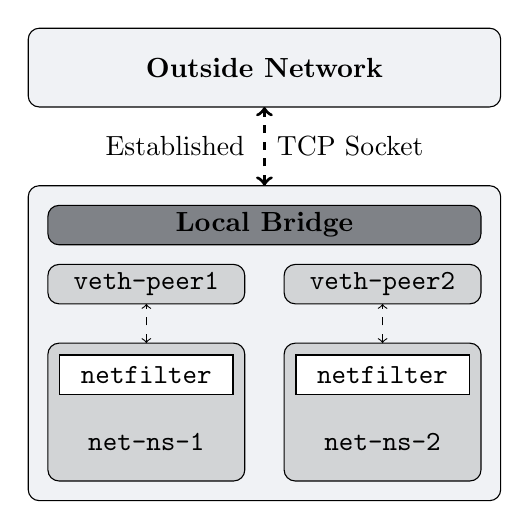
\begin{tikzpicture}
        % Color definition
        \definecolor{machineBG}{RGB}{240, 242, 245}
        \definecolor{namespaceBG}{RGB}{210, 212, 214}
        \definecolor{bridgeBG}{RGB}{127, 130, 135}

        % Host network box
        \draw[fill=machineBG, rounded corners] (0,0) rectangle (6, 4);
        % Network Namespace 1 and Peer
        \draw[fill=namespaceBG, rounded corners] (0.25, 0.25) rectangle (2.75, 2.0);
        \node at (1.5, 0.75) {\textbf{\texttt{net-ns-1}}};
        \draw[fill=white] (0.4, 1.35) rectangle (2.6, 1.85) node[pos=.5] {\text{\texttt{netfilter}}};
        \draw[<->, dashed] (1.5,2) -- (1.5,2.5);
        \draw[fill=namespaceBG, rounded corners] (0.25, 2.5) rectangle (2.75, 3) node[pos=.5] {\text{\texttt{veth-peer1}}};
        % Network Namespace 2
        \draw[fill=namespaceBG, rounded corners] (3.25, 0.25) rectangle (5.75, 2.0);
        \node at (4.5, 0.75) {\textbf{\texttt{net-ns-2}}};
        \draw[fill=white] (3.4, 1.35) rectangle (5.6, 1.85) node[pos=.5] {\text{\texttt{netfilter}}};
        \draw[<->, dashed] (4.5,2) -- (4.5,2.5);
        \draw[fill=namespaceBG, rounded corners] (3.25, 2.5) rectangle (5.75, 3) node[pos=.5] {\text{\texttt{veth-peer2}}};
        % Local Bridge
        \draw[fill=bridgeBG, rounded corners] (0.25, 3.25) rectangle (5.75, 3.75) node[pos=.5] {\textbf{Local Bridge}};

        % Connecting line
        \draw[<->, dashed, very thick] (3,4) -- (3,5) node[pos=.5] {Established \hspace{5pt} TCP Socket};

        % Outside network box
        \draw[fill=machineBG, rounded corners] (0,5) rectangle (6, 6) node[pos=.5] {\textbf{Outside Network}};
    \end{tikzpicture}
    \caption{Architecture of three different namespaces connected through virtual ethernet pairs.\label{fig:veth-arch}}
\end{figure}

Integration with \runc is two-fold.
For the TCP connection \criu's binding for \runc includes a \texttt{--tcp-established} flag that does most of the socket management.
If we are interested in restoring the connection in a different machine or namespace, we must manually recreate the filter table from Table~\ref{table:iptables-rules} using the \texttt{iptables} command.
Lastly, to restore into an existing namespace, the container must be restored with the adequate open file descriptors using \criu's \texttt{--external}~\cite{criu-external} and \texttt{--inherit-fd}~\cite{criu-inherit-fd}.
In Listings~\ref{code:microbenchmark-tcp-nonetns} and~\ref{code:microbenchmark-tcp-netns} we include excerpts of snippets to checkpoint and restore an established TCP connection without or within a network namespace respectively.
The complete scripts for the evaluation are included in Listings~\ref{code:microbenchmark-tcp-criu-downtime} and~\ref{code:microbenchmark-tcp-criu-reactivity} for \criu's downtime and reactivity experiments, and in Listings~\ref{code:microbenchmark-tcp-runc-downtime} and~\ref{code:microbenchmark-tcp-runc-reactivity} for \runc's.
\begin{figure}[h!]
\begin{minipage}{.45\textwidth}
\begin{lstlisting}[style=Bash,caption={Checkpoint and restore an established TCP connection using \criu and \runc.\label{code:microbenchmark-tcp-nonetns}}]
#!/bin/bash
# CRIU Dump and Restore, one after the other 
# but in the BG (not affecting time)
(sudo criu dump \
    -t ${SERVER_PID} \
    --images-dir ${IMAGES_DIR} \
    --tcp-established; \
echo "Restoring server..."; \
sudo criu restore \
    --images-dir ${IMAGES_DIR} \
    --tcp-established) &

# Similarly with runC
(sudo runc checkpoint \
    --image-path ${IMAGES_DIR} \
    --tcp-established \
    eureka; \
cd /container/directory; \
sudo runc restore \
    --image-path ${IMAGES_DIR} \
    --tcp-established \
    eureka; \
cd ${CWD}) &
\end{lstlisting}
\end{minipage}\hfill
\begin{minipage}{.45\textwidth}
\begin{lstlisting}[style=Bash,caption={Excerpt of a script to checkpoint a connection within an existing namespace, and inherit it on restore.\label{code:microbenchmark-tcp-netns}}]
#!/bin/bash
# Two namespaces with path NS_1 and NS_2
INO_1=$(ls -iL ${NS_1} | awk '{ print $1 }')
INO_2=$(ls -iL ${NS_2} | awk '{ print $1 }')
exec 33< ${NS_1}
exec 34< ${NS_2}

# To checkpoint we mark as an external
# resource both NS
sudo criu dump \
    -t ${PID_1} \
    --images-dir images \
    --tcp-established \
    --external net[${INO_1}]:${NS_1} \
    --external net[${INO_2}]:${NS_2}

# At restore, we match the file 
# descriptors with the NS
sudo criu restore \
    --images-dir images \
    --tcp-established \
    --inherit-fd fd[33]:${NS_1} \
    --inherit-fd fd[34]:${NS_2} -d
\end{lstlisting}
\end{minipage}
\end{figure}

\textbf{Benchmarking}

In order to evaluate the impact of migrating a process with an established TCP connection, we are interested in assessing how quickly can communication resume after restore.

To achieve this goal we set up the following testbed.
We first deploy two identical virtual machines running Linux Debian with kernel version \texttt{4.19.0-6}.
Each one has \criu version 3.13 and \runc version \texttt{1.0.0-rc8}, both built from source.
Additionally, and in order to conduct the experiments, we make use of \texttt{iPerf3} (version \texttt{3.7+}) a network bandwidth benchmarking tool~\cite{iperf3}.
In particular, we start an \texttt{iPerf3} client-server pair, one in each VM, and record the perceived throughput by the client.
Each experiment is repeated running the bare processes and checkpointing them using \criu, or isolating them within a \runc container, to assess the introduced overhead.
We measure from the client side since we are interested in dumping and restoring the server.
This situation makes more sense from the cloud-provider/load-balancing standpoint.

\textbf{Re-connection after a down period.}
The first experiment simulates the scenario in which the server is restored some time after the dump occured.
In particular, we let the client saturate the link for 10 seconds, then dump the server, and restore it 2 seconds later, all of which transparently to the client (whose connection is never closed).
In Figure~\ref{fig:evaluation-downtime} we present the throughput perceived by the client as a function of time. 
\begin{figure}[h!]
    \centering
    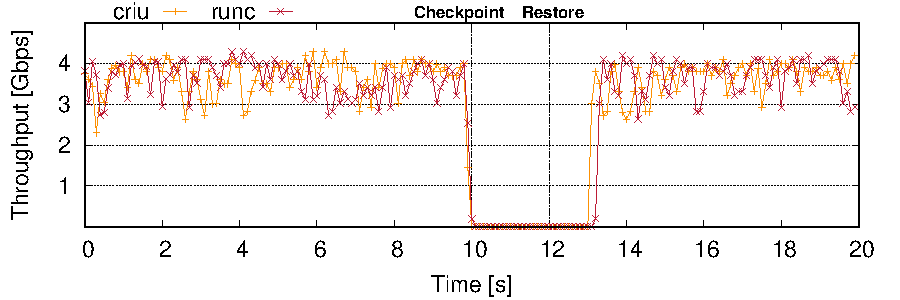
\includegraphics[width=\linewidth]{./figs/tcp-established-downtime/tcp_established_downtime_microbenchmark.pdf}
    \caption{Throughput perceived from the client as a function of time, when we checkpoint the server once, and restore it after two seconds. We compare the results of \criu and \runc. \label{fig:evaluation-downtime}}
\end{figure}
The first observation we make from the plot, is that it takes almost a full second to get the connection back to full speed.
To understand this behaviour we must recall what is \texttt{iPerf3} actually doing.
The client tries to saturate the link, sending as many packets as it can, and reports the measured capacity.
As the socket is never closed, and packets are just discarded by the network filters, to the client it will be as if those packets were never acknowledged, and hence will try to retransmit them.
The TCP protocol specifies~\cite{tcp-rfc} that the retransmission timeout must be doubled every time a packet is not acknowledged, therefore the recurrent outage of ACKs might cause the client to back-off for the perceived full second.
This implies that checkpointing established TCP connections only makes sense in the scenario in which the service is soon going to be restored.
The next experiment tackles the behaviour under this situation.

\textbf{Reactivity to immediate restore.}
To prove our hypothesis that the large delay after a restore is due to the protocol itself rather than our implementation, we set up an experiment in which we perform a sequence of dumps and immediate restores of the same established TCP connection.
We again present the throughput as a function of time in Figure~\ref{fig:evaluation-reactivity}.
\begin{figure}[h!]
    \centering
    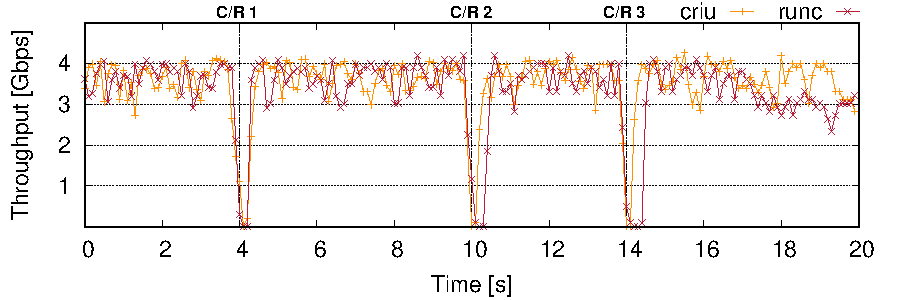
\includegraphics[width=\linewidth]{./figs/tcp-established-resolution/tcp_established_resolution_microbenchmark.pdf}
    \caption{Throughput from the client as a function of time.\label{fig:evaluation-reactivity}}
\end{figure}
In this case the measured throughput downtime does not exceed $0.1$ seconds, an order of magnitude better than the previous experiment.
This reduced value, together with the fact that the application studied is very network-intensive, makes us believe that our proposed technique is suitable for most client-server scenarios and won't have an impact in the overall quality of service.

Lastly, in both Figures we observe that, albeit being the experiments running bare processes with \criu slightly faster to restore, the overhead introduced by \runc is negligible.

To be done.
\jg{The previous sentence must be probably a comment}
A necessary first step is to manage the namespaces and IPs as we do now.

\section{Putting it All Together} \label{sec:system}

\cs{Cover the current implementation}

\cs{Include some code snippets/design choices}


\chapter{Evaluation} \label{chap:evaluation}

In the previous chapter, \S\ref{chap:system}, we have presented our implementation of live migration of containers using \criu and \runc, and have motivated our design choices with micro-benchmarks that fulfil the initial objectives specified in the introduction.

In this chapter, we move on to evaluate the system as a whole, and how the different features interlace and work together, and  how does our system compare to traditional virtual machine live migration.

\section{Macro-Benchmarks}

\subsection{Iterative, Remote, Diskless Migration}

Goal here would be to have the diagram we went over once, in which we plot over time the amount of memory we send.

\cs{Re-do the initial plot presented}

\subsection{Checkpointing TCP Connections inside Network Namespaces}

\cs{Include the content from Decentralized Systems}

\section{Comparison with Virtual Machines Migration}

\section{Scalability}

\begin{figure}
    \centering
    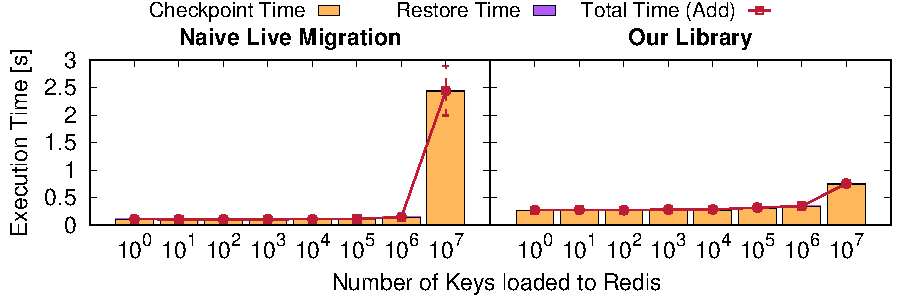
\includegraphics[width=\textwidth]{figs/key-scalability/key_scalability.pdf}
    \caption[Scalability with respect to the memory to transfer.]{Scalability with respect to the memory to transfer. We compare our system with manual live migration when running in the same machine with a one-shot migration.\label{fig:key-scalability}}
\end{figure}

\cs{Downtime as we increase the number of iterations (i.e. threshold)}

\cs{Comparison with VM Teleport}

\begin{lstlisting}[style=Bash,caption={Script to teleport a VirtualBox VM, and run the macrobenchmark.},label={code:vm-teleport}]
#!/bin/bash

# Configure target machine to wait for a teleport request to arrive
VBoxManage modifyvm 'CRIU-Debian-Teleport-Target' --teleporter on --teleporterport 6000

# Iterate over the different number of keys
for num_keys in 1 10 100 1000 10000 100000 1000000 10000000
do
    # Start the host machine as usual
    ssh <HOST_VM>
    cd ~/runc-containers/redis && ./run_redis.sh 100000

    # Start the target machine, if using a normal start, a process dialog will appear

    # Run the migration
    time VBoxManage controlvm 'CRIU-Debian' teleport --host localhost --port 6000

    # Shut down both VMs
done
\end{lstlisting}

\cs{Compare with P-Haul if time}

%\chapter{\projName in the Real World} \label{chap:applications}

The aim of this chapter would be to choose a couple of applications (maybe Redis DB and VPN server) motivate their need, introduce the scenario, why is our project useful and run a realistic evaluation.

For each section I would like to have:
\begin{itemize}
    \item Small Introduction of the scenario and the motivation.
    \item Description of the parts w/ a graphic and experiments
    \item Some graphics displaying results.
\end{itemize}

\cs{This is the part that still needs the most work.}

\section{Web Scenario: Database, Web Server, and Client}


\section{Remote Work Setting: VPN Server, Database, and Client}

\section{Containers in Scientific Computation}

Maybe try and use our system in an environment in which various nodes are working in parallel towards doing a computation, and we checkpoint the whole thing (with the dependencies) do some sort of manta inane or run another higher priority job, and then resume the original one.

%\chapter{Future Work} \label{chap:future-work}


\chapter{Conclusions and Future Work} \label{chap:conclusion}



% Bibliography: for the different bibliography styles see https://www.overleaf.com/learn/latex/Bibtex_bibliography_styles
%\pagebreak
\bibliographystyle{unsrt}
\bibliography{biblio}

\begin{appendices}
	\chapter{Implementation Code Snippets} \label{chap:app-code}

\begin{lstlisting}[language=C,caption={Simple counter in C.},label={code:c-counter}]
#include <signal.h>
#include <stdio.h>
#include <stdlib.h> /* atoi */
#include <unistd.h>

static volatile int keep_running = 1;

/* Handler to graciously stop with Ctrl+C */
void int_handler(int tmp)
{
    keep_running = 0;
}

/* Compile with: gcc counter.c -o counter */
int main(int argc, char *argv[])
{
    int count = 0;
    int inc = 0;
    if (argc > 1)
        inc = atoi(argv[1]);
    signal(SIGINT, int_handler);

    fprintf(stdout, "Current count: %i\n", count++);
    if (inc)
    {
        while (keep_running)
        {
            fprintf(stdout, "Current count: %i\n", count++);
            sleep(2);
        }
    }
    else 
    {
        while (keep_running)
            sleep(20);
    }

    return 0;
}
\end{lstlisting}

\begin{lstlisting}[language=C,caption={Signature and schematic implementation of remote execution methods.\label{code:libssh}}]
int sftp_copy_file(ssh_session session, char *dst_path, char *src_path)
{
    sftp_session sftp;
    int rc;

    sftp = sftp_new(session);
    /* Allocate SFTP Session */
    if (sftp == NULL)
    {
        fprintf(stderr, "sftp_copy_file: Error allocating SFTP session: %s\n",
                ssh_get_error(session));
        return SSH_ERROR;
    }

    /* Initialize SFTP Client */
    rc = sftp_init(sftp);
    if (rc != SSH_OK)
    {
        fprintf(stderr, "sftp_copy_file: Error initializing SFTP session: %d\n",
                sftp_get_error(sftp));
        sftp_free(sftp);
        return rc;
    }

    if (sftp_xfer_file(sftp, dst_path, src_path, NULL) != SSH_OK)
        return SSH_ERROR;

    sftp_free(sftp);
    return SSH_OK;
}

/* Copy the Contents of the Source Directory to the Destination One 
 *
 * ssh_session session: current authenticated ssh_session.
 * char *dst_path: path to the (existing) destination directory.
 * char *ori_path: path to the (existing) origin directory from where to copy.
 * int rm_ori: if set to 1, it will remove the contents of the origin directory.
 * int *dir_size: if not null, will return the size of the dir xfered.
 */
int sftp_copy_dir(ssh_session session, char *dst_path, char *src_path,
                  int rm_ori, double *dir_size)
{
    sftp_session sftp;
    int rc;

    sftp = sftp_new(session);
    /* Allocate SFTP Session */
    if (sftp == NULL)
    {
        fprintf(stderr, "sftp_copy_dir: Error allocating SFTP session: %s\n",
                ssh_get_error(session));
        return SSH_ERROR;
    }

    /* Initialize SFTP Client */
    rc = sftp_init(sftp);
    if (rc != SSH_OK)
    {
        fprintf(stderr, "sftp_copy_dir: Error initializing SFTP session: %d\n",
                sftp_get_error(sftp));
        sftp_free(sftp);
        return rc;
    }

    /* Iterate over source directory. */
    DIR *d;
    struct dirent *src_dir;
    //struct stat src_stat;
    d = opendir(src_path);
    if (d)
    {
        /* Create remote copy of directory. */
        /* TODO make this optional?
        if (sftp_mkdir(sftp, dst_path, 0755) != 0)
        {
            fprintf(stderr, "sftp_copy_dir: Error creating remore directory %d\n",
                    sftp_get_error(sftp));
            sftp_free(sftp);
            return SSH_ERROR;
        }
        */
        char resolved_path[PATH_MAX + 1];
        char src_rel_path[PATH_MAX + 1], dst_rel_path[PATH_MAX + 1];
        memset(src_rel_path, '\0', PATH_MAX + 1);
        memset(dst_rel_path, '\0', PATH_MAX + 1);
        memset(resolved_path, '\0', PATH_MAX + 1);
        while ((src_dir = readdir(d)) != NULL)
        {
            if (src_dir->d_type == DT_REG)
            {
                /* Generate full paths */
                strncpy(src_rel_path, src_path, strlen(src_path));
                strcat(src_rel_path, "/");
                strcat(src_rel_path, src_dir->d_name);
                strncpy(dst_rel_path, dst_path, strlen(dst_path));
                strcat(dst_rel_path, "/");
                strcat(dst_rel_path, src_dir->d_name);
                if (realpath(src_rel_path, resolved_path) == NULL)
                {
                    fprintf(stderr, "sftp_copy_dir: Error obtaining file's real path: %s\n",
                            src_dir->d_name);
                    sftp_free(sftp);
                    return SSH_ERROR;
                }
                if (sftp_xfer_file(sftp, dst_rel_path, resolved_path, dir_size)
                        != SSH_OK)
                {
                    fprintf(stderr, "sftp_copy_dir: error copying %s \
                                     to %s\n. %i\n", resolved_path,
                                     dst_rel_path, sftp_get_error(sftp));
                    sftp_free(sftp);
                    return SSH_ERROR;
                }
                if (rm_ori && remove(resolved_path) != 0)
                {
                    fprintf(stderr, "sftp_copy_dir: error removing local \
                                     file %s (remove flag set)\n",
                                     resolved_path);
                    sftp_free(sftp);
                    return SSH_ERROR;
                }
                memset(src_rel_path, '\0', PATH_MAX + 1);
                memset(dst_rel_path, '\0', PATH_MAX + 1);
                memset(resolved_path, '\0', PATH_MAX + 1);
            }
            else if (src_dir->d_type == DT_LNK)
            {
                /* On iterative migration, each intermediate checkpoint dir
                 * has a symbolic link to its "parent". Copying it
                 * programatically is more verbose than crafting it ourselves.
                 */
                strncpy(src_rel_path, src_path, strlen(src_path));
                strcat(src_rel_path, "/");
                strcat(src_rel_path, src_dir->d_name);
                if (remove(src_rel_path) != 0)
                {
                    fprintf(stderr, "sftp_copy_dir: error removing \
                                     symlink.\n");
                    return 1;
                }
                memset(src_rel_path, '\0', PATH_MAX + 1);
            }
        }
        closedir(d);
    }
    else
    {
        fprintf(stderr, "sftp_copy_dir: Error listing source directory!\n");
        sftp_free(sftp);
        return SSH_ERROR;
    }

    if (rm_ori && (rmdir(src_path) != 0))
    {
        fprintf(stderr, "sftp_copy_dir: failed removing origin directory \
                         '%s'\n", src_path);
        sftp_free(sftp);
        return SSH_ERROR;
    }
    sftp_free(sftp);
    return SSH_OK;
}
\end{listing}
int ssh_remote_command(ssh_session session, char *command, int read_output)
{
    ssh_channel channel;
    int rc;
    char buffer[256];
    int nbytes;

    /* Open a new SSH Channel */
    channel = ssh_channel_new(session);
    if (channel == NULL)
    {
        fprintf(stderr, "ssh_remote_command: Error allocating new SSH channel.\n");
        return SSH_ERROR;
    }
    rc = ssh_channel_open_session(channel);
    if (rc != SSH_OK)
    {
        fprintf(stderr, "ssh_remote_command: Error opening new SSH channel.\n");
        ssh_channel_free(channel);
        return rc;
    }

    /* Execute Remote Command 
     *
     * We need to run the commands as sudo in the remote system as well
     * (criu needs to run as root) so I thought of two different ways
     * of tackling the problem:
     * 1. Passing the password as plain text.
     * 2. Manually setup each host to allow rootless sudo.
     * */
    /*
    char sudo_command[MAX_CMD_SIZE];
    memset(sudo_command, '\0', MAX_CMD_SIZE);
    sprintf(sudo_command, "echo %s | sudo -S %s", REMOTE_PWRD, command);
    */
    rc = ssh_channel_request_exec(channel, command);
    if (rc != SSH_OK)
    {
        fprintf(stderr, "ssh_remote_command: Error executing remote command: %s\n",
                command);
        ssh_channel_close(channel);
        ssh_channel_free(channel);
        return rc;
    }

    /* Check the Exit Status of the Remote Command */
    rc = ssh_channel_get_exit_status(channel);
    switch (rc) 
    {
        case 0:
            printf("DEBUG: command '%s' exitted succesfully!\n", command);
            break;

        case -1:
            printf("DEBUG: still no exit code received!\n");
            break;

        default:
            fprintf(stderr, "ssh_remote_command: remote command '%s' failed w/ exit status %i\n",
                    command, rc);
            return SSH_ERROR;
    }

    if (read_output)
    {
        /* Read Output in chunks */
        nbytes = ssh_channel_read(channel, buffer, sizeof buffer, 0);
        while(nbytes > 0)
        {
            fprintf(stdout, "%s", buffer);
            /* FIXME check for errors
            if (fprintf(stdout, "%s", buffer) != (unsigned int) nbytes)
            {
                fprintf(stderr, "Error printing results.\n");
                ssh_channel_close(channel);
                ssh_channel_free(channel);
                return SSH_ERROR;
            }
            */
            nbytes = ssh_channel_read(channel, buffer, sizeof buffer, 0);
        }
        
        if (nbytes < 0)
        {
            ssh_channel_close(channel);
            ssh_channel_free(channel);
            return SSH_ERROR;
        }
    }

    ssh_channel_send_eof(channel);
    ssh_channel_close(channel);
    ssh_channel_free(channel);
    return SSH_OK;
}

int sftp_copy_file(ssh_session session, char *dst_path, char *src_path)
{
    sftp_session sftp;
    int rc;

    sftp = sftp_new(session);
    /* Allocate SFTP Session */
    if (sftp == NULL)
    {
        fprintf(stderr, "sftp_copy_file: Error allocating SFTP session: %s\n",
                ssh_get_error(session));
        return SSH_ERROR;
    }

    /* Initialize SFTP Client */
    rc = sftp_init(sftp);
    if (rc != SSH_OK)
    {
        fprintf(stderr, "sftp_copy_file: Error initializing SFTP session: %d\n",
                sftp_get_error(sftp));
        sftp_free(sftp);
        return rc;
    }

    if (sftp_xfer_file(sftp, dst_path, src_path, NULL) != SSH_OK)
        return SSH_ERROR;

    sftp_free(sftp);
    return SSH_OK;
}

/* Copy the Contents of the Source Directory to the Destination One 
 *
 * ssh_session session: current authenticated ssh_session.
 * char *dst_path: path to the (existing) destination directory.
 * char *ori_path: path to the (existing) origin directory from where to copy.
 * int rm_ori: if set to 1, it will remove the contents of the origin directory.
 * int *dir_size: if not null, will return the size of the dir xfered.
 */
int sftp_copy_dir(ssh_session session, char *dst_path, char *src_path,
                  int rm_ori, double *dir_size)
{
    sftp_session sftp;
    int rc;

    sftp = sftp_new(session);
    /* Allocate SFTP Session */
    if (sftp == NULL)
    {
        fprintf(stderr, "sftp_copy_dir: Error allocating SFTP session: %s\n",
                ssh_get_error(session));
        return SSH_ERROR;
    }

    /* Initialize SFTP Client */
    rc = sftp_init(sftp);
    if (rc != SSH_OK)
    {
        fprintf(stderr, "sftp_copy_dir: Error initializing SFTP session: %d\n",
                sftp_get_error(sftp));
        sftp_free(sftp);
        return rc;
    }

    /* Iterate over source directory. */
    DIR *d;
    struct dirent *src_dir;
    //struct stat src_stat;
    d = opendir(src_path);
    if (d)
    {
        /* Create remote copy of directory. */
        /* TODO make this optional?
        if (sftp_mkdir(sftp, dst_path, 0755) != 0)
        {
            fprintf(stderr, "sftp_copy_dir: Error creating remore directory %d\n",
                    sftp_get_error(sftp));
            sftp_free(sftp);
            return SSH_ERROR;
        }
        */
        char resolved_path[PATH_MAX + 1];
        char src_rel_path[PATH_MAX + 1], dst_rel_path[PATH_MAX + 1];
        memset(src_rel_path, '\0', PATH_MAX + 1);
        memset(dst_rel_path, '\0', PATH_MAX + 1);
        memset(resolved_path, '\0', PATH_MAX + 1);
        while ((src_dir = readdir(d)) != NULL)
        {
            if (src_dir->d_type == DT_REG)
            {
                /* Generate full paths */
                strncpy(src_rel_path, src_path, strlen(src_path));
                strcat(src_rel_path, "/");
                strcat(src_rel_path, src_dir->d_name);
                strncpy(dst_rel_path, dst_path, strlen(dst_path));
                strcat(dst_rel_path, "/");
                strcat(dst_rel_path, src_dir->d_name);
                if (realpath(src_rel_path, resolved_path) == NULL)
                {
                    fprintf(stderr, "sftp_copy_dir: Error obtaining file's real path: %s\n",
                            src_dir->d_name);
                    sftp_free(sftp);
                    return SSH_ERROR;
                }
                if (sftp_xfer_file(sftp, dst_rel_path, resolved_path, dir_size)
                        != SSH_OK)
                {
                    fprintf(stderr, "sftp_copy_dir: error copying %s \
                                     to %s\n. %i\n", resolved_path,
                                     dst_rel_path, sftp_get_error(sftp));
                    sftp_free(sftp);
                    return SSH_ERROR;
                }
                if (rm_ori && remove(resolved_path) != 0)
                {
                    fprintf(stderr, "sftp_copy_dir: error removing local \
                                     file %s (remove flag set)\n",
                                     resolved_path);
                    sftp_free(sftp);
                    return SSH_ERROR;
                }
                memset(src_rel_path, '\0', PATH_MAX + 1);
                memset(dst_rel_path, '\0', PATH_MAX + 1);
                memset(resolved_path, '\0', PATH_MAX + 1);
            }
            else if (src_dir->d_type == DT_LNK)
            {
                /* On iterative migration, each intermediate checkpoint dir
                 * has a symbolic link to its "parent". Copying it
                 * programatically is more verbose than crafting it ourselves.
                 */
                strncpy(src_rel_path, src_path, strlen(src_path));
                strcat(src_rel_path, "/");
                strcat(src_rel_path, src_dir->d_name);
                if (remove(src_rel_path) != 0)
                {
                    fprintf(stderr, "sftp_copy_dir: error removing \
                                     symlink.\n");
                    return 1;
                }
                memset(src_rel_path, '\0', PATH_MAX + 1);
            }
        }
        closedir(d);
    }
    else
    {
        fprintf(stderr, "sftp_copy_dir: Error listing source directory!\n");
        sftp_free(sftp);
        return SSH_ERROR;
    }

    if (rm_ori && (rmdir(src_path) != 0))
    {
        fprintf(stderr, "sftp_copy_dir: failed removing origin directory \
                         '%s'\n", src_path);
        sftp_free(sftp);
        return SSH_ERROR;
    }
    sftp_free(sftp);
    return SSH_OK;
}
\end{lstlisting}

\chapter{Evaluation Code Snippets} \label{chap:app:evaluation}

\begin{lstlisting}[style=Bash,caption={Full evaluation script for the diskless migration micro-benchmark using. \label{code:microbenchmark-diskless-evaluation}}]
#!/bin/bash
HOME=$(pwd)
#IP=127.0.0.1
IP=192.168.56.103
NUM_TESTS=100
acc=0
acc2=0
for (( i=1; i<=$NUM_TESTS; i++ ))
do
    # Choose application to run
    #cd /home/carlos/runc-containers/counter/ && sudo ./run.sh && cd $HOME
    cd /home/carlos/runc-containers/redis/ && sudo ./run_redis.sh 10000000 && cd $HOME
    # Clean working Environment
    sudo ./clean.sh
    ssh carlos@${IP} "/home/carlos/runc-diskless/clean.sh"
    # Start (or not) the page server
    #sudo ./page_server.sh &
    #ssh carlos@${IP} "/home/carlos/runc-diskless/page_server.sh &> /dev/null < /dev/null &"
    # Start timing
    ts=$(date +%s%N)
    # Dump the process
    sudo ./dump.sh
    # Copy the remaining images
    #scp -r ./src-images/* ./dst-images/
    scp -r ./src-images/* carlos@${IP}:runc-diskless/dst-images/
    time_elapsed=$((($(date +%s%N) - $ts)/1000000))
    acc=$(($acc + $time_elapsed))
    acc2=$(($acc2 + $time_elapsed * $time_elapsed))
    echo "Test $i: $time_elapsed"
done
# Compute average and standard deviation
avg=$(bc <<<"scale=2; $acc / $NUM_TESTS")
std=$(bc <<<"scale=2; sqrt($acc2 / $NUM_TESTS - $avg * $avg)")
echo "Average: $avg"
echo "Std: $std"
\end{lstlisting}

\begin{lstlisting}[style=Bash,caption={Full evaluation script for the iterative migration micro-benchmark.\label{code:microbenchmark-iterative-evaluation}}]
#!/bin/bash
# Run Process
# Redis Test (Pre-loading omitted)
redis_server --port 9999 &> /dev/null < /dev/null &
# Counter Test
sudo ./counter &> /dev/null < /dev/null &
# If running with runC
cd container-dir && sudo runc run -d container_name &> /dev/null < /dev/null & && cd -
PID=$!

# Clean Environment
sudo ./clean.sh
echo "Clean Done"

# First pre-dump
sudo ./pre-dump.sh ${PID}
echo "Pre-Dump Done"

# If running the Redis test, run the benchmark
redis-benchmark -p 9999 -n 10000 &> /dev/null

# Second pre-dump
sudo ./middle-dump.sh ${PID}
echo "Middle-Dump Done"

# If running the Redis test, run the benchmark
redis-benchmark -p 9999 -n 10000 &> /dev/null

# Last Dump
sudo ./dump.sh ${PID}
echo "Dump Done"

# Print results
D1=$(ls -lah ./images/1/pages-1.img | awk '{ print $5; }')
D2=$(ls -lah ./images/2/pages-1.img | awk '{ print $5; }')
D3=$(ls -lah ./images/3/pages-1.img | awk '{ print $5; }')
echo "Test finished: -D1: $D1 -D2: $D2 -D3: $D3"
\end{lstlisting}

\begin{lstlisting}[style=Bash,caption={Full evaluation script for the tcp connection downtime microbenchmark using \criu.\label{code:microbenchmark-tcp-criu-downtime}}]
#!/bin/bash
# Declare Variables
CLIENT_IP=192.168.56.103
IPERF3=/home/carlos/iperf/src/iperf3
LOG_DIR=./iperf3-log
IMAGES_DIR=./images

# Set up Environment
mkdir -p ${LOG_DIR}

# Run iPerf3 server
echo "Bootstrapping Server..."
setsid ${IPERF3} \
    -s --port 9999 \
    --json \
    --interval 0.1 \
    --logfile ${LOG_DIR}/server.json \
    --one-off &> /dev/null < /dev/null &
SERVER_PID=$!

sleep 3

# Run iPerf3 client in remote machine
echo "Bootstrapping Client..."
ssh carlos@${CLIENT_IP} "/home/carlos/tcp-established/iperf3_client.sh"

sleep 10

# CRIU Dump
echo "Dumping server..."
sudo criu dump \
    -t ${SERVER_PID} \
    --images-dir ${IMAGES_DIR} \
    --tcp-established &

sleep 2

# CRIU Restore
echo "Restoring server..."
sudo criu restore \
    --images-dir ${IMAGES_DIR} \
    --tcp-established
\end{lstlisting}

\begin{lstlisting}[style=Bash,caption={Full evaluation script for the tcp connection reactivity microbenchmark using \criu.\label{code:microbenchmark-tcp-criu-reactivity}}]
#!/bin/bash
# Declare Variables
CLIENT_IP=192.168.56.103
IPERF3=/home/carlos/iperf/src/iperf3
LOG_DIR=./iperf3-log
IMAGES_DIR=./images

# Set up Environment
mkdir -p ${LOG_DIR}

# Run iPerf3 server
echo "Bootstrapping Server..."
setsid ${IPERF3} \
    -s --port 9999 \
    --json \
    --interval 0.1 \
    --logfile ${LOG_DIR}/server.json \
    --one-off &> /dev/null < /dev/null &
SERVER_PID=$!

sleep 3

# Run iPerf3 client in remote machine
echo "Bootstrapping Client..."
ssh carlos@${CLIENT_IP} "/home/carlos/tcp-established/iperf3_client.sh"

sleep 4

# CRIU Dump and Restore, one after the other but in the BG (not affecting time)
echo "Dumping server for the first time..."
(sudo criu dump \
    -t ${SERVER_PID} \
    --images-dir ${IMAGES_DIR} \
    --tcp-established; \
echo "Restoring server..."; \
sudo criu restore \
    --images-dir ${IMAGES_DIR} \
    --tcp-established) &

sleep 6

# CRIU Dump and Restore, one after the other but in the BG (not affecting time)
echo "Dumping server for the second time..."
(sudo criu dump \
    -t ${SERVER_PID} \
    --images-dir ${IMAGES_DIR} \
    --tcp-established; \
echo "Restoring server..."; \
sudo criu restore \
    --images-dir ${IMAGES_DIR} \
    --tcp-established) &

sleep 4

# CRIU Dump and Restore, one after the other but in the BG (not affecting time)
echo "Dumping server for the last time..."
(sudo criu dump \
    -t ${SERVER_PID} \
    --images-dir ${IMAGES_DIR} \
    --tcp-established; )
echo "Restoring server..."; \
sudo criu restore \
    --images-dir ${IMAGES_DIR} \
    --tcp-established)
\end{lstlisting}

\begin{lstlisting}[style=Bash,caption={Full evaluation script for the tcp connection downtime microbenchmark using \runc.\label{code:microbenchmark-tcp-runc-downtime}}]
#!/bin/bash
# Declare Variables
CLIENT_IP=192.168.56.103
IPERF3=/home/carlos/iperf/src/iperf3
LOG_DIR=./iperf3-log
IMAGES_DIR=/home/carlos/criu-lm/experiments/tcp-established/images
CWD=$(pwd)

# Set up Environment
mkdir -p ${LOG_DIR}

# Run iPerf3 server
cd /home/carlos/runc-containers/iperf3-server
sudo runc run eureka &> /dev/null < /dev/null &
cd ${CWD}

sleep 3

# Run iPerf3 client in remote machine
echo "Bootstrapping Client..."
ssh carlos@${CLIENT_IP} "/home/carlos/tcp-established/iperf3_client.sh"

sleep 10

# CRIU Dump
echo "Dumping server..."
sudo runc checkpoint \
    --image-path ${IMAGES_DIR} \
    --tcp-established \
    eureka

sleep 2

# CRIU Restore
echo "Restoring server..."
cd /home/carlos/runc-containers/iperf3-server 
sudo runc restore \
    --image-path ${IMAGES_DIR} \
    --tcp-established \
    eureka-restored
cd ${CWD}
\end{lstlisting}

\begin{lstlisting}[style=Bash,caption={Full evaluation script for the tcp connection reactivity microbenchmark using \runc.\label{code:microbenchmark-tcp-runc-reactivity}}]
#!/bin/bash
# Declare Variables
CLIENT_IP=192.168.56.103
IPERF3=/home/carlos/iperf/src/iperf3
LOG_DIR=./iperf3-log
IMAGES_DIR=/home/carlos/criu-lm/experiments/tcp-established/images
CWD=$(pwd)

# Set up Environment
mkdir -p ${LOG_DIR}

# Run iPerf3 server
cd /home/carlos/runc-containers/iperf3-server
sudo runc run eureka &> /dev/null < /dev/null &
cd ${CWD}

sleep 3

# Run iPerf3 client in remote machine
echo "Bootstrapping Client..."
ssh carlos@${CLIENT_IP} "/home/carlos/tcp-established/iperf3_client.sh"

sleep 4

# CRIU Dump
echo "Dumping server..."
(sudo runc checkpoint \
    --image-path ${IMAGES_DIR} \
    --tcp-established \
    eureka; \
cd /home/carlos/runc-containers/iperf3-server; \
sudo runc restore \
    --image-path ${IMAGES_DIR} \
    --tcp-established \
    eureka; \
cd ${CWD}) &

sleep 6

# CRIU Dump
echo "Dumping server..."
(sudo runc checkpoint \
    --image-path ${IMAGES_DIR} \
    --tcp-established \
    eureka; \
cd /home/carlos/runc-containers/iperf3-server; \
sudo runc restore \
    --image-path ${IMAGES_DIR} \
    --tcp-established \
    eureka; \
cd ${CWD}) &

sleep 4

# CRIU Dump
echo "Dumping server..."
(sudo runc checkpoint \
    --image-path ${IMAGES_DIR} \
    --tcp-established \
    eureka; \
cd /home/carlos/runc-containers/iperf3-server; \
sudo runc restore \
    --image-path ${IMAGES_DIR} \
    --tcp-established \
    eureka; \
cd ${CWD})
\end{lstlisting}

\end{appendices}

\end{document}
